\documentclass{extbook}[14pt]
\usepackage{multicol, enumerate, enumitem, hyperref, color, soul, setspace, parskip, fancyhdr, amssymb, amsthm, amsmath, bbm, latexsym, units, mathtools}
\everymath{\displaystyle}
\usepackage[headsep=0.5cm,headheight=0cm, left=1 in,right= 1 in,top= 1 in,bottom= 1 in]{geometry}
\usepackage{dashrule}  % Package to use the command below to create lines between items
\newcommand{\litem}[1]{\item #1

\rule{\textwidth}{0.4pt}}
\pagestyle{fancy}
\lhead{}
\chead{Answer Key for Progress Quiz 4 Version B}
\rhead{}
\lfoot{8448-1521}
\cfoot{}
\rfoot{Fall 2020}
\begin{document}
\textbf{This key should allow you to understand why you choose the option you did (beyond just getting a question right or wrong). \href{https://xronos.clas.ufl.edu/mac1105spring2020/courseDescriptionAndMisc/Exams/LearningFromResults}{More instructions on how to use this key can be found here}.}

\textbf{If you have a suggestion to make the keys better, \href{https://forms.gle/CZkbZmPbC9XALEE88}{please fill out the short survey here}.}

\textit{Note: This key is auto-generated and may contain issues and/or errors. The keys are reviewed after each exam to ensure grading is done accurately. If there are issues (like duplicate options), they are noted in the offline gradebook. The keys are a work-in-progress to give students as many resources to improve as possible.}

\rule{\textwidth}{0.4pt}

\begin{enumerate}\litem{
Describe the zero behavior of the zero $x = -6$ of the polynomial below.
\[ f(x) = -6(x - 6)^{9}(x + 6)^{14}(x + 3)^{6}(x - 3)^{9} \]
The solution is the graph below, which is option B.
\begin{center}
    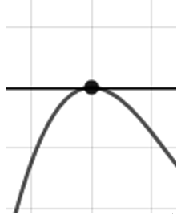
\includegraphics[width=0.3\textwidth]{../Figures/polyZeroBehaviorCopyBB.png}
\end{center}\begin{enumerate}[label=\Alph*.]
\begin{multicols}{2}
\item 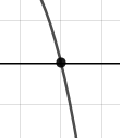
\includegraphics[width = 0.3\textwidth]{../Figures/polyZeroBehaviorCopyAB.png}
\item 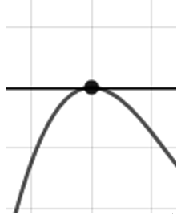
\includegraphics[width = 0.3\textwidth]{../Figures/polyZeroBehaviorCopyBB.png}
\item 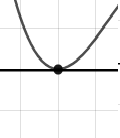
\includegraphics[width = 0.3\textwidth]{../Figures/polyZeroBehaviorCopyCB.png}
\item 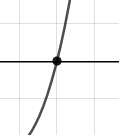
\includegraphics[width = 0.3\textwidth]{../Figures/polyZeroBehaviorCopyDB.png}
\end{multicols}\item None of the above.\end{enumerate}
\textbf{General Comment:} You will need to sketch the entire graph, then zoom in on the zero the question asks about.
}
\litem{
Which of the following equations \textit{could} be of the graph presented below?

\begin{center}
    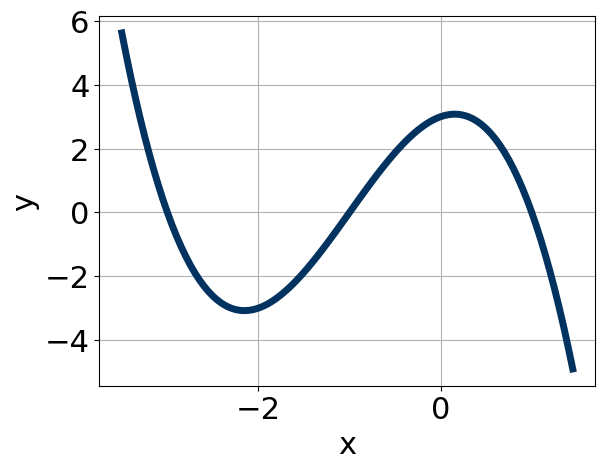
\includegraphics[width=0.5\textwidth]{../Figures/polyGraphToFunctionB.png}
\end{center}



The solution is \( -15(x + 3)^{10} (x - 3)^{6} (x + 2)^{11} \), which is option D.\begin{enumerate}[label=\Alph*.]
\item \( 17(x + 3)^{10} (x - 3)^{8} (x + 2)^{7} \)

This corresponds to the leading coefficient being the opposite value than it should be.
\item \( -10(x + 3)^{6} (x - 3)^{7} (x + 2)^{7} \)

The factor $(x - 3)$ should have an even power.
\item \( -8(x + 3)^{6} (x - 3)^{9} (x + 2)^{8} \)

The factor $(x - 3)$ should have an even power and the factor $(x + 2)$ should have an odd power.
\item \( -15(x + 3)^{10} (x - 3)^{6} (x + 2)^{11} \)

* This is the correct option.
\item \( 19(x + 3)^{4} (x - 3)^{6} (x + 2)^{10} \)

The factor $(x + 2)$ should have an odd power and the leading coefficient should be the opposite sign.
\end{enumerate}

\textbf{General Comment:} General Comments: Draw the x-axis to determine which zeros are touching (and so have even multiplicity) or cross (and have odd multiplicity).
}
\litem{
Describe the end behavior of the polynomial below.
\[ f(x) = 2(x - 9)^{2}(x + 9)^{3}(x - 2)^{4}(x + 2)^{6} \]
The solution is the graph below, which is option D.
\begin{center}
    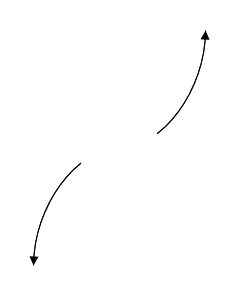
\includegraphics[width=0.3\textwidth]{../Figures/polyEndBehaviorDB.png}
\end{center}\begin{enumerate}[label=\Alph*.]
\begin{multicols}{2}
\item 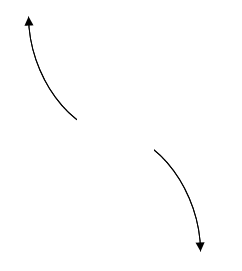
\includegraphics[width = 0.3\textwidth]{../Figures/polyEndBehaviorAB.png}
\item 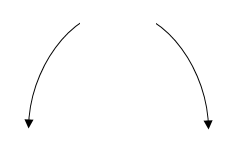
\includegraphics[width = 0.3\textwidth]{../Figures/polyEndBehaviorBB.png}
\item 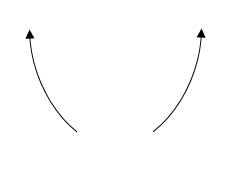
\includegraphics[width = 0.3\textwidth]{../Figures/polyEndBehaviorCB.png}
\item 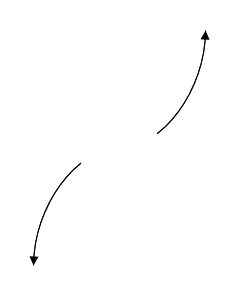
\includegraphics[width = 0.3\textwidth]{../Figures/polyEndBehaviorDB.png}
\end{multicols}\item None of the above.\end{enumerate}
\textbf{General Comment:} Remember that end behavior is determined by the leading coefficient AND whether the \textbf{sum} of the multiplicities is positive or negative.
}
\litem{
Which of the following equations \textit{could} be of the graph presented below?

\begin{center}
    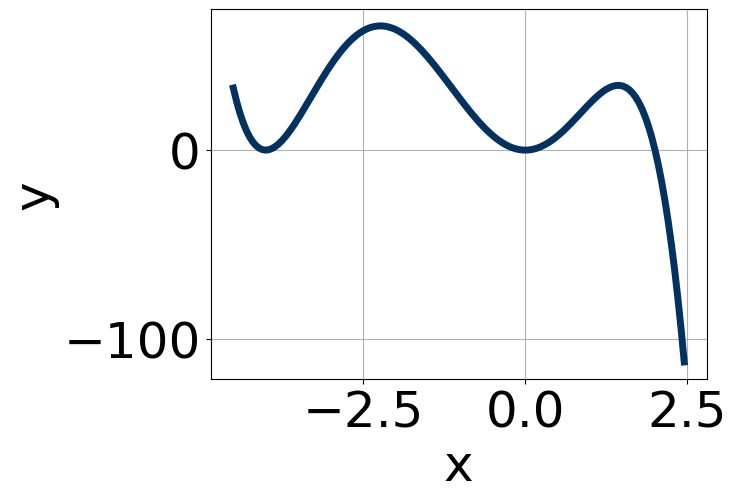
\includegraphics[width=0.5\textwidth]{../Figures/polyGraphToFunctionCopyB.png}
\end{center}



The solution is \( 14x^{5} (x - 2)^{10} (x + 3)^{11} \), which is option C.\begin{enumerate}[label=\Alph*.]
\item \( 19x^{5} (x - 2)^{6} (x + 3)^{8} \)

The factor $(x + 3)$ should have an odd power.
\item \( -15x^{4} (x - 2)^{4} (x + 3)^{11} \)

The factor $x$ should have an odd power and the leading coefficient should be the opposite sign.
\item \( 14x^{5} (x - 2)^{10} (x + 3)^{11} \)

* This is the correct option.
\item \( 18x^{5} (x - 2)^{9} (x + 3)^{4} \)

The factor $2$ should have an even power and the factor $-3$ should have an odd power.
\item \( -15x^{11} (x - 2)^{6} (x + 3)^{5} \)

This corresponds to the leading coefficient being the opposite value than it should be.
\end{enumerate}

\textbf{General Comment:} General Comments: Draw the x-axis to determine which zeros are touching (and so have even multiplicity) or cross (and have odd multiplicity).
}
\litem{
Describe the end behavior of the polynomial below.
\[ f(x) = 6(x - 2)^{4}(x + 2)^{5}(x + 3)^{4}(x - 3)^{4} \]
The solution is the graph below, which is option D.
\begin{center}
    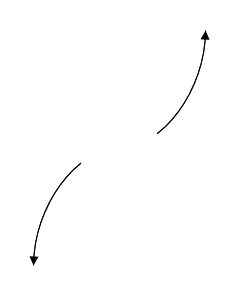
\includegraphics[width=0.3\textwidth]{../Figures/polyEndBehaviorCopyDB.png}
\end{center}\begin{enumerate}[label=\Alph*.]
\begin{multicols}{2}
\item 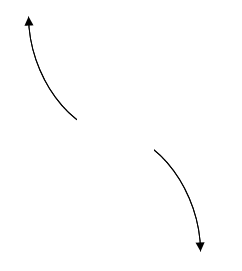
\includegraphics[width = 0.3\textwidth]{../Figures/polyEndBehaviorCopyAB.png}
\item 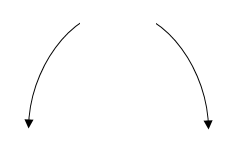
\includegraphics[width = 0.3\textwidth]{../Figures/polyEndBehaviorCopyBB.png}
\item 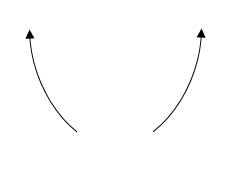
\includegraphics[width = 0.3\textwidth]{../Figures/polyEndBehaviorCopyCB.png}
\item 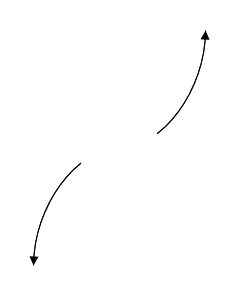
\includegraphics[width = 0.3\textwidth]{../Figures/polyEndBehaviorCopyDB.png}
\end{multicols}\item None of the above.\end{enumerate}
\textbf{General Comment:} Remember that end behavior is determined by the leading coefficient AND whether the \textbf{sum} of the multiplicities is positive or negative.
}
\litem{
Construct the lowest-degree polynomial given the zeros below. Then, choose the intervals that contain the coefficients of the polynomial in the form $ax^3+bx^2+cx+d$.
\[ -7, \frac{2}{3}, \text{ and } -2 \]
The solution is \( 3x^{3} +25 x^{2} +24 x -28 \), which is option D.\begin{enumerate}[label=\Alph*.]
\item \( a \in [-1, 5], b \in [-17.9, -15.3], c \in [-36, -27], \text{ and } d \in [27, 36] \)

$3x^{3} -17 x^{2} -32 x + 28$, which corresponds to multiplying out $(x + 1)(3x -3)(x -1)$.
\item \( a \in [-1, 5], b \in [23.4, 27.8], c \in [22, 26], \text{ and } d \in [27, 36] \)

$3x^{3} +25 x^{2} +24 x + 28$, which corresponds to multiplying everything correctly except the constant term.
\item \( a \in [-1, 5], b \in [-13.7, -11.2], c \in [-60, -51], \text{ and } d \in [-30, -25] \)

$3x^{3} -13 x^{2} -52 x -28$, which corresponds to multiplying out $(x + 1)(3x + 3)(x -1)$.
\item \( a \in [-1, 5], b \in [23.4, 27.8], c \in [22, 26], \text{ and } d \in [-30, -25] \)

* $3x^{3} +25 x^{2} +24 x -28$, which is the correct option.
\item \( a \in [-1, 5], b \in [-27.3, -24], c \in [22, 26], \text{ and } d \in [27, 36] \)

$3x^{3} -25 x^{2} +24 x + 28$, which corresponds to multiplying out $(x -7)(3x + 2)(x -2)$.
\end{enumerate}

\textbf{General Comment:} To construct the lowest-degree polynomial, you want to multiply out $(x + 7)(3x -2)(x + 2)$
}
\litem{
Construct the lowest-degree polynomial given the zeros below. Then, choose the intervals that contain the coefficients of the polynomial in the form $ax^3+bx^2+cx+d$.
\[ \frac{-3}{2}, -3, \text{ and } \frac{1}{3} \]
The solution is \( 6x^{3} +25 x^{2} +18 x -9 \), which is option A.\begin{enumerate}[label=\Alph*.]
\item \( a \in [2, 7], b \in [24, 32], c \in [16, 21], \text{ and } d \in [-16, -2] \)

* $6x^{3} +25 x^{2} +18 x -9$, which is the correct option.
\item \( a \in [2, 7], b \in [-25, -22], c \in [16, 21], \text{ and } d \in [6, 10] \)

$6x^{3} -25 x^{2} +18 x + 9$, which corresponds to multiplying out $(2x -3)(x -3)(3x + 1)$.
\item \( a \in [2, 7], b \in [-32, -27], c \in [32, 43], \text{ and } d \in [-16, -2] \)

$6x^{3} -29 x^{2} +36 x -9$, which corresponds to multiplying out $(2x + 2)(x + 1)(3x -3)$.
\item \( a \in [2, 7], b \in [24, 32], c \in [16, 21], \text{ and } d \in [6, 10] \)

$6x^{3} +25 x^{2} +18 x + 9$, which corresponds to multiplying everything correctly except the constant term.
\item \( a \in [2, 7], b \in [6, 8], c \in [-30, -29], \text{ and } d \in [6, 10] \)

$6x^{3} +7 x^{2} -30 x + 9$, which corresponds to multiplying out $(2x + 2)(x -1)(3x -3)$.
\end{enumerate}

\textbf{General Comment:} To construct the lowest-degree polynomial, you want to multiply out $(2x + 3)(x + 3)(3x -1)$
}
\litem{
Construct the lowest-degree polynomial given the zeros below. Then, choose the intervals that contain the coefficients of the polynomial in the form $x^3+bx^2+cx+d$.
\[ -5 + 2 i \text{ and } -4 \]
The solution is \( x^{3} +14 x^{2} +69 x + 116 \), which is option B.\begin{enumerate}[label=\Alph*.]
\item \( b \in [-10, 3], c \in [8, 16], \text{ and } d \in [14, 22] \)

$x^{3} + x^{2} +9 x + 20$, which corresponds to multiplying out $(x + 5)(x + 4)$.
\item \( b \in [8, 18], c \in [62, 78], \text{ and } d \in [116, 124] \)

* $x^{3} +14 x^{2} +69 x + 116$, which is the correct option.
\item \( b \in [-22, -9], c \in [62, 78], \text{ and } d \in [-118, -111] \)

$x^{3} -14 x^{2} +69 x -116$, which corresponds to multiplying out $(x-(-5 + 2 i))(x-(-5 - 2 i))(x -4)$.
\item \( b \in [-10, 3], c \in [-2, 3], \text{ and } d \in [-14, -5] \)

$x^{3} + x^{2} +2 x -8$, which corresponds to multiplying out $(x -2)(x + 4)$.
\item \( \text{None of the above.} \)

This corresponds to making an unanticipated error or not understanding how to use nonreal complex numbers to create the lowest-degree polynomial. If you chose this and are not sure what you did wrong, please contact the coordinator for help.
\end{enumerate}

\textbf{General Comment:} Remember that the conjugate of $a+bi$ is $a-bi$. Since these zeros always come in pairs, we need to multiply out $(x-(-5 + 2 i))(x-(-5 - 2 i))(x-(-4))$.
}
\litem{
Describe the zero behavior of the zero $x = -4$ of the polynomial below.
\[ f(x) = -8(x - 4)^{8}(x + 4)^{11}(x + 9)^{3}(x - 9)^{4} \]
The solution is the graph below, which is option A.
\begin{center}
    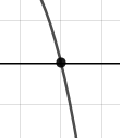
\includegraphics[width=0.3\textwidth]{../Figures/polyZeroBehaviorAB.png}
\end{center}\begin{enumerate}[label=\Alph*.]
\begin{multicols}{2}
\item 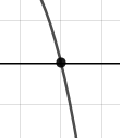
\includegraphics[width = 0.3\textwidth]{../Figures/polyZeroBehaviorAB.png}
\item 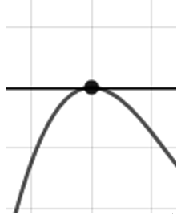
\includegraphics[width = 0.3\textwidth]{../Figures/polyZeroBehaviorBB.png}
\item 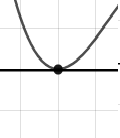
\includegraphics[width = 0.3\textwidth]{../Figures/polyZeroBehaviorCB.png}
\item 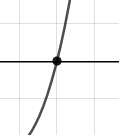
\includegraphics[width = 0.3\textwidth]{../Figures/polyZeroBehaviorDB.png}
\end{multicols}\item None of the above.\end{enumerate}
\textbf{General Comment:} You will need to sketch the entire graph, then zoom in on the zero the question asks about.
}
\litem{
Construct the lowest-degree polynomial given the zeros below. Then, choose the intervals that contain the coefficients of the polynomial in the form $x^3+bx^2+cx+d$.
\[ -5 + 5 i \text{ and } -1 \]
The solution is \( x^{3} +11 x^{2} +60 x + 50 \), which is option A.\begin{enumerate}[label=\Alph*.]
\item \( b \in [7, 17], c \in [58, 67], \text{ and } d \in [46, 54] \)

* $x^{3} +11 x^{2} +60 x + 50$, which is the correct option.
\item \( b \in [-15, -6], c \in [58, 67], \text{ and } d \in [-50, -44] \)

$x^{3} -11 x^{2} +60 x -50$, which corresponds to multiplying out $(x-(-5 + 5 i))(x-(-5 - 5 i))(x -1)$.
\item \( b \in [-4, 5], c \in [4, 7], \text{ and } d \in [1, 6] \)

$x^{3} + x^{2} +6 x + 5$, which corresponds to multiplying out $(x + 5)(x + 1)$.
\item \( b \in [-4, 5], c \in [-10, -3], \text{ and } d \in [-16, 1] \)

$x^{3} + x^{2} -4 x -5$, which corresponds to multiplying out $(x -5)(x + 1)$.
\item \( \text{None of the above.} \)

This corresponds to making an unanticipated error or not understanding how to use nonreal complex numbers to create the lowest-degree polynomial. If you chose this and are not sure what you did wrong, please contact the coordinator for help.
\end{enumerate}

\textbf{General Comment:} Remember that the conjugate of $a+bi$ is $a-bi$. Since these zeros always come in pairs, we need to multiply out $(x-(-5 + 5 i))(x-(-5 - 5 i))(x-(-1))$.
}
\end{enumerate}

\end{document}